% !TEX TS-program = pdflatex
% !TEX encoding = UTF-8 Unicode

\chapter{Introduction} \label{chapter:intro}

	\pagenumbering{arabic}

	\section{Student Memoirs}

When I was a student I often left bits of electronic circuitry
in my pockets, such as \newacronym{led}{LED}{light-emitting diode}\glspl{led}\index{led} and \newacronym{eeprom}{EEPROM}{electrically erasable programmable read-only memory}\index{eeprom}, which
often ended up in the washing machine. The \glspl{led}\index{led} didn't
fair too badly, but the \glspl{eeprom}\index{eeprom} frequently broke \cite{citRef2}. One \gls{led}, two \glspl{led} \cite{citRef1}.

\subsection{Symbols}

The \newglossaryentry{angstrom}{type=symbols,name={\aa}ngstr\"om,symbol={\AA},sort=angstrom, description={non-SI unit of length}}\gls{angstrom} is commonly used in structural biology,
whereas the \newglossaryentry{ohm}{type=symbols,name=ohm,symbol={\ensuremath{\Omega}},description=unit of electrical resistance}\gls{ohm} is used in electronics \cite{citRef2,citRef3}.
	
	\subsubsection{Test 1}
	
	In Figure \ref{fig:mesh1} we can see a mesh !!!
	
	\begin{figure}[h]
    		\centering
    		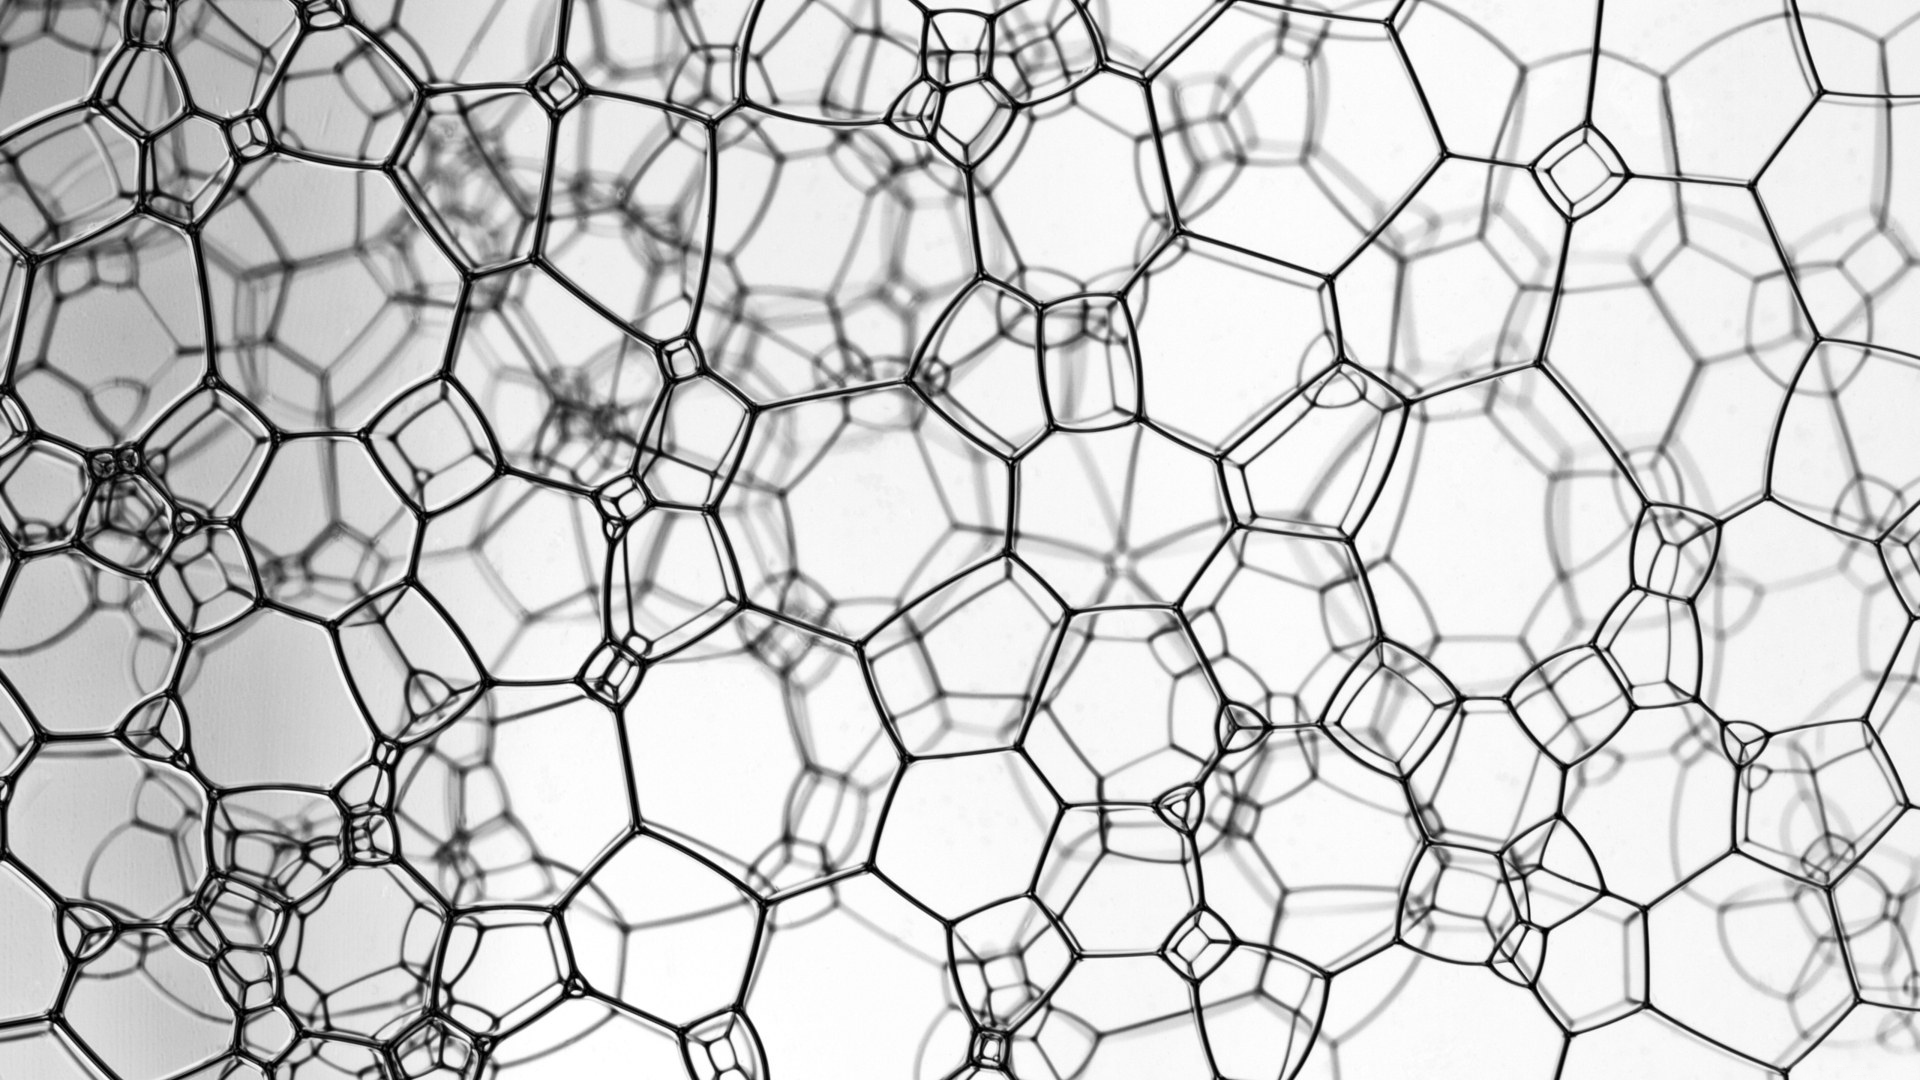
\includegraphics[width=0.5\textwidth]{../images/introduction/mesh}
    		\caption{A nice plot}
    		\label{fig:mesh1}
	\end{figure}
	
	\subsubsection{Test 2}
	
	Table \ref{tab:example1} is just an example and has nothing to do with \glspl{led}\index{led}. 
	
	\begin{table}[h]
	    \begin{tabular} {|c|c||>{\centering}p{.9cm}|>{\centering}p{.9cm}|>{\centering}p{.9cm}|c|}
	        \hline
	        \emph{Truth} & \emph{Predicted} & ADA & SVM & GLM & Blended \\ \hline
	        T & T & 512 & 463 & 423 & 472 \\ 
	        T & F & 19  & 68  & 108 & 0   \\ 
	        F & T & 5   & 85  & 67  & 22  \\ 
	        F & F & 580 & 500 & 518 & 98  \\ \hline
	    \end{tabular} \\ \vskip .5cm
	
	    \begin{tabular} {>{\centering}p{2.9cm}dddd}
	        \toprule
	        \textit{Accuracy Metric} & \textrm{ADA} & \textrm{SVM} & \textrm{GLM} & \textrm{Blended} \\ \midrule
	        Precision & 99.0\% & 84.5\% & 86.3\% & 95.57\% \\ 
	        Recall    & 96.4\% & 87.2\% & 79.7\% & 100.0\%  \\
	        Accuracy  & 97.8\% & 86.3\% & 84.3\% & 96.3\% \\ \bottomrule
	    \end{tabular} 
	
	    \caption{Truth Tables and Accuracy Measures for each modeling library.}
	    \label{tab:example1}   
	\end{table}
	
	\subsubsection{Test 3}
	
	An example of a function plot using the ``tikz'' package:
	


\lipsum
	
	